\documentclass[12pt,a4paper]{article}

% ─── Page Layout ───────────────────────────────────────────────────────────────
\usepackage[a4paper, margin=0.8in, headheight=14pt]{geometry}

% ─── Fonts (XeLaTeX) ───────────────────────────────────────────────────────────
\usepackage{fontspec}
\usepackage{unicode-math}
\setmainfont{TeX Gyre Pagella}
\setmonofont[Scale=0.88]{TeX Gyre Cursor}
\setmathfont{Latin Modern Math}

% ─── Packages ──────────────────────────────────────────────────────────────────
\usepackage{xcolor}
\usepackage{colortbl}
\usepackage{titlesec}
\usepackage{enumitem}
\usepackage{tabularx}
\usepackage{booktabs}
\usepackage{array}
\usepackage{amsmath}
\usepackage{tikz}
\usetikzlibrary{shapes.geometric, arrows.meta, positioning, calc, fit, decorations.pathreplacing}
\usepackage{tcolorbox}
\tcbuselibrary{skins, breakable}
\usepackage{hyperref}
\usepackage{fancyhdr}
\usepackage{graphicx}
\usepackage{microtype}
\hyphenpenalty=10000
\exhyphenpenalty=10000
\sloppy
\usepackage{caption}
\usepackage{setspace}
\usepackage{multirow}
\usepackage{tocloft}

% ─── Q&A helper ────────────────────────────────────────────────────────────────
\newcommand{\Q}[1]{\textbf{#1}\par\noindent\ignorespaces}

% ─── Colour Palette ────────────────────────────────────────────────────────────
\definecolor{myred}{RGB}{196,30,58}
\definecolor{mydark}{RGB}{30,30,50}
\definecolor{mygreen}{RGB}{14,120,80}
\definecolor{myteal}{RGB}{0,130,140}
\definecolor{myamber}{RGB}{180,100,0}
\definecolor{mypurple}{RGB}{100,30,160}
\definecolor{mygray}{RGB}{246,247,249}
\definecolor{mgframe}{RGB}{180,185,200}
\definecolor{watermark}{RGB}{145,150,170}
\definecolor{hdrred}{RGB}{250,232,235}
\definecolor{hdrgreen}{RGB}{220,244,233}
\definecolor{hdrteal}{RGB}{220,242,244}
\definecolor{hdramber}{RGB}{253,242,215}
\definecolor{hdrpurple}{RGB}{238,228,255}
\definecolor{hdrgray}{RGB}{238,240,245}
\definecolor{rowalt}{RGB}{250,251,253}

% ─── Section Formatting ────────────────────────────────────────────────────────
\titleformat{\section}
  {\large\bfseries\color{myred}}{\thesection.}{0.5em}{}
  [\vspace{1pt}{\color{myred}\rule{\linewidth}{0.8pt}}]
\titleformat{\subsection}
  {\normalsize\bfseries\color{myteal}}{\thesubsection}{0.5em}{}
\titlespacing*{\section}{0pt}{18pt}{7pt}
\titlespacing*{\subsection}{0pt}{11pt}{4pt}

% ─── Paragraph ─────────────────────────────────────────────────────────────────
\setlength{\parindent}{0pt}
\setlength{\parskip}{4pt}

% ─── TOC Styling ───────────────────────────────────────────────────────────────
\renewcommand{\cfttoctitlefont}{\large\bfseries\color{myred}}
\renewcommand{\cftaftertoctitle}{\par\noindent{\color{myred}\rule{\linewidth}{0.8pt}}}
\setlength{\cftbeforetoctitleskip}{0pt}
\setlength{\cftaftertoctitleskip}{6pt}
\renewcommand{\cftsecfont}{\normalsize\bfseries\color{mydark}}
\renewcommand{\cftsecpagefont}{\normalsize\bfseries\color{mydark}}
\renewcommand{\cftsecleader}{\cftdotfill{\cftdotsep}}
\setlength{\cftbeforesecskip}{7pt}
\renewcommand{\cftsubsecfont}{\small\color{mydark}}
\renewcommand{\cftsubsecpagefont}{\small\color{mydark}}
\setlength{\cftbeforesubsecskip}{3pt}
\setlength{\cftsubsecindent}{1.4em}

% ─── Table helpers ─────────────────────────────────────────────────────────────
\renewcommand{\arraystretch}{1.45}
\setlength{\tabcolsep}{6pt}
\arrayrulecolor{mydark}
\newcolumntype{B}[1]{>{\small\bfseries\raggedright\arraybackslash}m{#1}}
\newcolumntype{Y}{>{\small\raggedright\arraybackslash}X}
\renewcommand{\tabularxcolumn}[1]{m{#1}}

% ─── Header / Footer ───────────────────────────────────────────────────────────
\pagestyle{fancy}
\fancyhf{}
\fancyhead[L]{\small\color{myred}\textbf{OE-EC604C}\;\color{mydark}--- Object Oriented Programming}
\fancyhead[R]{\small\color{myteal}\textbf{Module 2 Notes}}
\fancyfoot[C]{\small\color{mydark}\thepage}
\fancyfoot[R]{\small\color{watermark}\textit{\copyright\ Biraj}}
\renewcommand{\headrulewidth}{0.5pt}
\renewcommand{\footrulewidth}{0.3pt}

% ─── Hyperref ──────────────────────────────────────────────────────────────────
\hypersetup{
  colorlinks=true, linkcolor=myteal, urlcolor=myteal,
  pdfauthor={Biraj Sarkar},
  pdftitle={OE-EC604C --- Module 2 Notes}
}

% ─── tcolorbox styles ──────────────────────────────────────────────────────────
\tcbset{
  tikzbox/.style={
    colback=mygray, colframe=mgframe, boxrule=0.6pt, arc=4pt,
    left=8pt, right=8pt, top=6pt, bottom=6pt,
    colbacktitle=mgframe, coltitle=mydark,
    fonttitle=\small\bfseries
  },
  defbox/.style={
    colback=hdrgreen, colframe=mygreen, boxrule=0.8pt, arc=4pt,
    left=9pt, right=9pt, top=6pt, bottom=6pt,
    colbacktitle=mygreen, coltitle=white,
    fonttitle=\small\bfseries
  },
  formulabox/.style={
    colback=hdrteal, colframe=myteal, boxrule=0.8pt, arc=4pt,
    left=9pt, right=9pt, top=7pt, bottom=7pt,
    colbacktitle=myteal, coltitle=white,
    fonttitle=\small\bfseries
  },
  examplebox/.style={
    colback=hdramber, colframe=myamber, boxrule=0.8pt, arc=4pt,
    left=9pt, right=9pt, top=6pt, bottom=6pt,
    colbacktitle=myamber, coltitle=white,
    fonttitle=\small\bfseries
  },
  masonbox/.style={
    colback=hdrpurple, colframe=mypurple, boxrule=0.8pt, arc=4pt,
    left=9pt, right=9pt, top=6pt, bottom=6pt,
    colbacktitle=mypurple, coltitle=white,
    fonttitle=\small\bfseries
  },
  exambox/.style={
    colback=hdrpurple, colframe=mypurple, boxrule=1pt, arc=5pt,
    left=10pt, right=10pt, top=8pt, bottom=8pt,
    colbacktitle=mypurple, coltitle=white,
    fonttitle=\bfseries,
    breakable, title after break={\textbf{Frequently Asked / Viva Questions (contd.)}}}
}
% Make all boxes breakable across pages
\tcbset{breakable}

% ─── TikZ styles ───────────────────────────────────────────────────────────────
\tikzset{
  block/.style={rectangle, draw=myteal, fill=hdrteal,
    text width=2.4cm, align=center, minimum height=0.95cm,
    font=\small, rounded corners=3pt, line width=0.7pt},
  redblock/.style={rectangle, draw=myred, fill=hdrred,
    text width=2.4cm, align=center, minimum height=0.95cm,
    font=\small, rounded corners=3pt, line width=0.7pt},
  netnode/.style={rectangle, draw=myteal, fill=hdrteal,
    text width=1.5cm, align=center, minimum height=0.8cm,
    font=\small, rounded corners=3pt, line width=0.7pt},
  sumjunc/.style={circle, draw=myamber, fill=hdramber,
    minimum size=0.62cm, font=\small, line width=0.8pt},
  snode/.style={circle, draw=mypurple, fill=hdrpurple,
    minimum size=0.55cm, font=\footnotesize, line width=0.7pt},
  arrow/.style={-Stealth, thick, color=mydark},
  redarrow/.style={-Stealth, thick, color=myred},
  line/.style={thick, color=mydark}
}

% ═══════════════════════════════════════════════════════════════════════════════
\begin{document}
% ═══════════════════════════════════════════════════════════════════════════════

\begin{center}
  {\LARGE\bfseries\color{myred} OE-EC604C --- Object Oriented Programming}\\[5pt]
  {\normalsize\color{mydark} Semester VI \quad$\bullet$\quad 3L:0T:0P \quad$\bullet$\quad 3 Credits}\\[3pt]
  {\normalsize\color{myteal}\textbf{Module 2 Exam Notes: Moving from C to C++}}\\[3pt]
  {\small\color{mydark} CGEC \;$|$\; B.Tech ECE (2023--27) \;$|$\; \textit{Biraj Sarkar}}
\end{center}
\vspace{2pt}
\noindent{\color{myred}\rule{\linewidth}{1.5pt}}
\vspace{2pt}

\hypersetup{linkcolor=mydark}
\tableofcontents
\hypersetup{linkcolor=myteal}
\newpage

% ===============================================================================
\section{C++ Streams, Namespaces \& Operators}
% ===============================================================================

C++ maintains backwards compatibility with C but introduces modern syntax and strict type checking to simplify development.

\subsection{Stream-Based Input/Output}
Unlike C which uses formatted functions like `printf` and `scanf`, C++ implements stream-based I/O. Streams are continuous sequences of bytes representing data flow.
\begin{itemize}[leftmargin=*, itemsep=3pt]
  \item \textbf{\texttt{cout}:} Standard output stream (connected to console), used with the stream insertion operator (\texttt{<<}).
  \item \textbf{\texttt{cin}:} Standard input stream (connected to keyboard), used with the stream extraction operator (\texttt{>>}).
  \item \textbf{Type Safety:} Operator overloading allows streams to automatically detect variables' data types (no format specifiers like \texttt{\%d} or \texttt{\%f} required).
\end{itemize}

\subsection{Namespaces}
\begin{tcolorbox}[defbox]
\textbf{Namespace:} A declarative region that provides a scope to the identifiers (names of types, functions, variables, etc.) inside it. Namespaces are used to organize code into logical groups and prevent name conflicts (clashing) in large projects.
\end{tcolorbox}
The C++ Standard Library is defined within a namespace named \textbf{\texttt{std}}. To use identifiers like `cout` or `cin`, we must specify their namespace:
\begin{align}
  &\text{using scope resolution: } \texttt{std::cout << "Hello";}\\
  &\text{using declaration: } \texttt{using std::cout; cout << "Hello";}\\
  &\text{using directive: } \texttt{using namespace std; cout << "Hello";}
\end{align}

\subsection{Scope Resolution Operator (\texttt{::})}
In C, if a local variable hides a global variable with the same name, there is no direct way to access the global variable. C++ introduces the scope resolution operator (\texttt{::}) to resolve scope conflicts.
\begin{tcolorbox}[formulabox, title={\textbf{Scope Resolution Syntax}}]
\begin{equation}
  \text{Global Variable Access: } \texttt{::variable\_name}
\end{equation}
It is also used for:
\begin{enumerate}[label=\alph*., leftmargin=1.5em, itemsep=1pt]
  \item Accessing static members of a class: \texttt{ClassName::static\_member}.
  \item Defining class member functions outside the class declaration.
  \item Resolving namespace paths: \texttt{NamespaceName::identifier}.
\end{enumerate}
\end{tcolorbox}

\begin{tcolorbox}[examplebox, title={Code Example: Global variable access via Scope Resolution}]
\begin{spacing}{1.0}
\begin{verbatim}
#include <iostream>
int x = 10; // Global variable
int main() {
    int x = 20; // Local variable hiding global x
    std::cout << "Local x = " << x << std::endl;      // Prints 20
    std::cout << "Global x = " << ::x << std::endl;    // Prints 10
    return 0;
}
\end{verbatim}
\end{spacing}
\end{tcolorbox}

\subsection{Variable Declaration and References}
\begin{itemize}[leftmargin=*, itemsep=3pt]
  \item \textbf{Declaration at Point of Use:} C requires variable declarations at the start of a block. C++ allows declaring variables anywhere in the code, immediately before their first use.
  \item \textbf{Reference Variables (Aliases):}
    \begin{tcolorbox}[defbox]
    \textbf{Reference Variable:} An alias or alternative name for an already existing variable. It shares the same memory space as the original variable. Modifying the reference modifies the original variable.
    \end{tcolorbox}
    \textbf{Declaration Syntax:}
    \begin{equation}
      \texttt{int x = 10; int \&y = x; // y is a reference to x}
    \end{equation}
    Reference variables must be initialized during declaration and cannot be re-bound to another variable.
\end{itemize}

% ===============================================================================
\section{Parameter Passing \& Functions}
% ===============================================================================

C++ extends function properties by introducing call-by-reference, inline compilation, and parameter defaults.

\subsection{Parameter Passing Mechanisms}
\begin{enumerate}[label=\textbf{\arabic*.}, leftmargin=*, itemsep=4pt]
  \item \textbf{Pass-by-Value:} A copy of the actual argument is passed to the function parameter. Changes inside the function do not affect the original variable.
  \item \textbf{Pass-by-Pointer:} The address of the argument is passed. The function dereferences the pointer to access/modify the original variable.
  \item \textbf{Pass-by-Reference:} The function parameter becomes an alias (reference) to the actual argument. No new memory is allocated, and the function directly manipulates the caller's variables.
\end{enumerate}

\begin{tcolorbox}[tikzbox, title={Memory Behavior of Parameter Passing}]
\centering
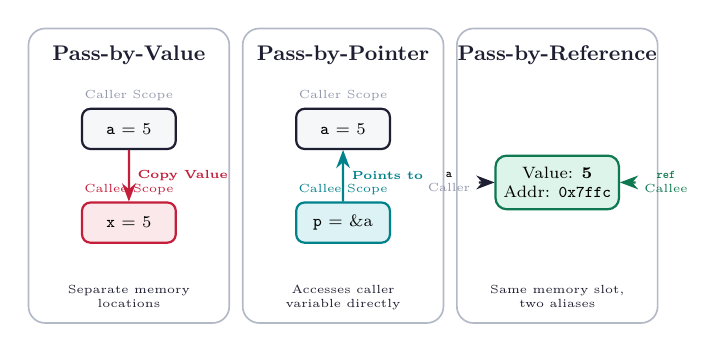
\begin{tikzpicture}[node distance=1.2cm, thick, scale=0.85, every node/.style={scale=0.85}]
  % Define styles locally
  \tikzset{
    varbox/.style={draw=mydark, fill=mygray, rounded corners=3pt, minimum width=1.4cm, minimum height=0.6cm, font=\scriptsize, align=center},
    card/.style={fill=white, draw=mgframe, rounded corners=6pt, line width=0.6pt}
  }

  % Pass-by-Value Card
  \draw[card] (-4.1, 2.2) rectangle (-1.1, -2.2);
  \node[font=\small\bfseries\color{mydark}] at (-2.6, 1.8) {Pass-by-Value};
  
  \node[font=\tiny\color{watermark}] at (-2.6, 1.2) {Caller Scope};
  \node[varbox] (val_caller) at (-2.6, 0.7) {\texttt{a} = 5};
  
  \node[font=\tiny\color{myred}] at (-2.6, -0.2) {Callee Scope};
  \node[varbox, draw=myred, fill=hdrred] (val_callee) at (-2.6, -0.7) {\texttt{x} = 5};
  
  \draw[arrow, color=myred] (val_caller) -- (val_callee) node[midway, right, font=\tiny\bfseries] {Copy Value};
  \node[below, font=\tiny\color{mydark}, align=center] at (-2.6, -1.5) {Separate memory\\locations};

  % Pass-by-Pointer Card
  \draw[card] (-0.9, 2.2) rectangle (2.1, -2.2);
  \node[font=\small\bfseries\color{mydark}] at (0.6, 1.8) {Pass-by-Pointer};
  
  \node[font=\tiny\color{watermark}] at (0.6, 1.2) {Caller Scope};
  \node[varbox] (ptr_caller) at (0.6, 0.7) {\texttt{a} = 5};
  
  \node[font=\tiny\color{myteal}] at (0.6, -0.2) {Callee Scope};
  \node[varbox, draw=myteal, fill=hdrteal] (ptr_callee) at (0.6, -0.7) {\texttt{p} = \&a};
  
  \draw[arrow, color=myteal] (ptr_callee) -- (ptr_caller) node[midway, right, font=\tiny\bfseries] {Points to};
  \node[below, font=\tiny\color{mydark}, align=center] at (0.6, -1.5) {Accesses caller\\variable directly};

  % Pass-by-Reference Card
  \draw[card] (2.3, 2.2) rectangle (5.3, -2.2);
  \node[font=\small\bfseries\color{mydark}] at (3.8, 1.8) {Pass-by-Reference};
  
  \node[draw=mygreen, fill=hdrgreen, rounded corners=4pt, minimum width=1.6cm, minimum height=0.8cm, font=\scriptsize, align=center] (ref_mem) at (3.8, -0.1) {Value: \textbf{5}\\Addr: \texttt{0x7ffc}};
  
  \node[left=0.2cm of ref_mem, align=center, font=\tiny] (ref_caller) {\textbf{\texttt{a}}\\\color{watermark}Caller};
  \node[right=0.2cm of ref_mem, align=center, font=\tiny\color{mygreen}] (ref_callee) {\textbf{\texttt{ref}}\\\color{mygreen}Callee};
  
  \draw[arrow] (ref_caller) -- (ref_mem.west);
  \draw[arrow, color=mygreen] (ref_callee) -- (ref_mem.east);
  
  \node[below, font=\tiny\color{mydark}, align=center] at (3.8, -1.5) {Same memory slot,\\two aliases};
\end{tikzpicture}
\end{tcolorbox}

\begin{tcolorbox}[examplebox, title={Code Example: Swapping variables using references}]
\begin{spacing}{1.0}
\begin{verbatim}
#include <iostream>
void swap(int &x, int &y) { // x and y are references to caller variables
    int temp = x;
    x = y;
    y = temp;
}
int main() {
    int a = 5, b = 10;
    swap(a, b); // Swaps values of a and b directly
    std::cout << "a = " << a << ", b = " << b; // Prints a = 10, b = 5
    return 0;
}
\end{verbatim}
\end{spacing}
\end{tcolorbox}

\subsection{Inline Functions}
Function calls introduce overhead: pushing arguments onto stack, saving registers, jumping to function address, restoring state on return. For small functions, the overhead can exceed the execution time of the function body.
\begin{tcolorbox}[defbox]
\textbf{Inline Function:} A function that is expanded in line at the point of call by the compiler instead of being invoked via standard function call stack jumps.
\end{tcolorbox}
\textbf{Syntax:}
\begin{equation}
  \texttt{inline int add(int a, int b) \{ return a + b; \}}
\end{equation}
\textbf{Key Rules and Compiler Discretion:}
The \texttt{inline} keyword is a \textbf{request}, not a command. The compiler can ignore it and compile the function normally if:
\begin{itemize}[leftmargin=*, itemsep=1pt, topsep=1pt]
  \item The function contains loops (\texttt{for}, \texttt{while}), switch statements, or goto.
  \item The function is recursive.
  \item The function contains static variables.
  \item The function returns a value but does not contain a return statement.
\end{itemize}

\subsection{Function Overloading}
Function overloading is a compile-time polymorphism feature allowing multiple functions to share the same name with different parameters.
\begin{tcolorbox}[defbox]
\textbf{Function Overloading:} The capability to declare multiple functions with the same name within the same scope, provided their signatures (parameter list) are unique.
\end{tcolorbox}
\textbf{Resolution Criteria:} The compiler distinguishes overloaded functions based on:
\begin{enumerate}[label=\textbf{\arabic*.}, leftmargin=1.5em, itemsep=1pt]
  \item \textbf{Number of parameters:} e.g., \texttt{void display(int)} vs \texttt{void display(int, int)}.
  \item \textbf{Type of parameters:} e.g., \texttt{void display(int)} vs \texttt{void display(double)}.
  \item \textbf{Order of parameters:} e.g., \texttt{void display(int, double)} vs \texttt{void display(double, int)}.
\end{enumerate}
\textbf{Note:} Functions cannot be overloaded based solely on their return types.

\subsection{Default Arguments}
Default arguments allow functions to assign a default value to a parameter if the caller does not provide an argument for it.
\textbf{Syntax:}
\begin{equation}
  \texttt{void printLine(char c = '*', int len = 40); // default values}
\end{equation}
\textbf{Critical Rule:}
Default arguments must be assigned from \textbf{right to left}. We cannot assign a default value to a parameter unless all parameters to its right also have default values.
\begin{align*}
  &\text{✅ Correct: } \texttt{void func(int a, int b = 10, int c = 20);}\\
  &\text{❌ Incorrect: } \texttt{void func(int a = 10, int b, int c = 20); // b lacks default}
\end{align*}

% ===============================================================================
% MANDATORY QUICK REVISION PAGE
% ===============================================================================
\newpage
\begin{center}
  {\large\bfseries\color{myred} Quick Revision --- Module II}\\[3pt]
  {\small\color{mydark} Moving from C to C++ $|$ OE-EC604C}
\end{center}
\noindent{\color{myred}\rule{\linewidth}{1.2pt}}
\vspace{4pt}

\begin{tcolorbox}[formulabox, title={\textbf{Key Formulas and Syntax}}]
\renewcommand{\arraystretch}{1.3}
\begin{tabularx}{\linewidth}{B{3.6cm} X}
Reference Variable      & \texttt{int x = 5; int \&ref = x; // ref shares memory with x} \\[4pt]
Inline Function         & \texttt{inline int square(int x) \{ return x * x; \}} \\[4pt]
Scope Resolution        & \texttt{::variable} \quad (accesses global variable hiding in local scope) \\[4pt]
Default Parameters      & \texttt{void value(int p, int n = 5, float r = 0.1); // right-to-left}
\end{tabularx}
\end{tcolorbox}

\begin{tcolorbox}[defbox, title={\textbf{One-Line Definitions}}]
\begin{itemize}[leftmargin=*, itemsep=2.5pt, topsep=0pt]
  \item \textbf{Reference Variable:} A constant pointer to variable that acts as an alternative name (alias) for that variable.
  \item \textbf{Namespace:} A scope region containing definitions to prevent name clashes in large programs.
  \item \textbf{Scope Resolution (::):} An operator used to access global variables or define class methods externally.
  \item \textbf{Inline Function:} A function that is compiled by replacing its calls directly with the function code.
  \item \textbf{Function Overloading:} Declaring multiple functions sharing the same name but unique parameters.
  \item \textbf{Default Argument:} A value assigned to a function parameter in its prototype used if argument is omitted.
  \item \textbf{Pass-by-Reference:} Passing parameters by sharing the caller's variable memory directly via references.
  \item \textbf{Type Safety:} Strict compile-time checks verifying variable types and function arguments matching.
\end{itemize}
\end{tcolorbox}

\begin{tcolorbox}[exambox, title={\textbf{Frequently Asked / Viva Questions}}]
\begin{enumerate}[topsep=0pt, label=\textbf{Q\arabic*.}, itemsep=5pt]
  \item \Q{Why does C++ input/output streams compile with greater type safety than C standard I/O?}
    C++ streams use overloaded insertion/extraction operators to automatically detect variable types, removing format specifier errors.
  \item \Q{Can we declare reference variables without initialization in C++?}
    No. A reference must be initialized to bind to a variable during declaration. E.g., `int \&ref;` causes a compile error.
  \item \Q{Can a reference variable be re-assigned to reference another variable later?}
    No. Once a reference variable is initialized to a target variable, it cannot be changed to reference any other variable.
  \item \Q{How does the scope resolution operator access global variables?}
    Adding the `::` prefix tells the compiler to search for the identifier in the global scope instead of the local stack block.
  \item \Q{What is the primary benefit of using inline functions?}
    It eliminates function call overhead (saving registers, jumping, stack frames), improving execution speed for small functions.
  \item \Q{Under what conditions will the C++ compiler ignore an inline request?}
    If the function is large, recursive, contains loops (`for`, `while`), switch/goto statements, or static variables.
  \item \Q{Can we overload a function based only on its return type?}
    No. The compiler resolves overloading by comparing parameter lists (number, type, order). Return types are ignored.
  \item \Q{State the mandatory rule for declaring default arguments in C++.}
    Default arguments must be added from right to left in the parameter list. No default argument can precede a non-default one.
  \item \Q{What is the difference between pass-by-pointer and pass-by-reference?}
    Pass-by-pointer passes a memory address (can be NULL, requires dereferencing). Pass-by-reference passes an alias (cannot be NULL, behaves like local variable).
  \item \Q{Explain the use of the `using namespace std;` statement.}
    It imports all identifiers from the standard library namespace (`std`) into global scope, removing the need to write `std::` prefixes.
  \item \Q{Why are inline functions preferred over preprocessor macros (\#define)?}
    Inline functions are compiled with full type-checking and follow scope and access rules, whereas macros are simple text replacements.
  \item \Q{What is a name collision/clash and how do namespaces solve it?}
    A name collision occurs when two libraries define classes or functions with identical names. Namespaces solve this by wrapping definitions in unique scope scopes.
\end{enumerate}
\tcbset{colbacktitle=mypurple, coltitle=white}
\end{tcolorbox}

\begin{tcolorbox}[tikzbox, title={Comparison of Parameter Passing Methods}]
\renewcommand{\arraystretch}{1.45}
\par\noindent
\begin{tabularx}{\linewidth}{|B{3.2cm}|Y|Y|Y|}
\hline
\textbf{Parameter} & \textbf{\color{myteal}Pass-by-Value} & \textbf{\color{myamber}Pass-by-Pointer} & \textbf{\color{mygreen}Pass-by-Reference} \\
\hline
\textbf{Memory Allocation} & Allocates new local storage for parameter copy. & Allocates storage for pointer address (4/8 bytes). & No new memory allocated. Shares caller's slot. \\
\hline
\textbf{Null Values} & Not applicable. & Pointer can be \texttt{nullptr}. & Reference cannot be null. \\
\hline
\textbf{Syntax} & Simple: \texttt{func(a)}. & Complex: \texttt{func(\&a)} and \texttt{*ptr}. & Simple: \texttt{func(a)} with parameter \texttt{\&ref}. \\
\hline
\textbf{Modifies Caller?} & No, operations are on copy. & Yes, via pointer dereferencing. & Yes, directly via alias. \\
\hline
\end{tabularx}
\end{tcolorbox}

\end{document}
